\documentclass[12pt,tikz]{standalone}
 
\usepackage{tkz-euclide}
\usetikzlibrary{shapes,backgrounds}

\newcommand\Star[3][]{%
		\path[#1] (0  :#3) -- ( 36:#2) 
		-- (72 :#3) -- (108:#2)
		-- (144:#3) -- (180:#2)
		-- (216:#3) -- (252:#2)
		-- (288:#3) -- (324:#2)--cycle;
	}
\newcommand\Center[3][]{
	\begin{scope}[shift = {(#2,#3)}, scale=0.010]
		\Star[#1]{2}{4}
	\end{scope}
	}
	
\newcommand\pointnnc[3][]{
	\begin{scope}[shift = {(#2,#3)}, scale=0.01]
		\draw[#1] (0,0) circle (1.5);
	\end{scope}
	}
\tikzstyle{arrow} = [thin,->,>=stealth]
 
\begin{document}
		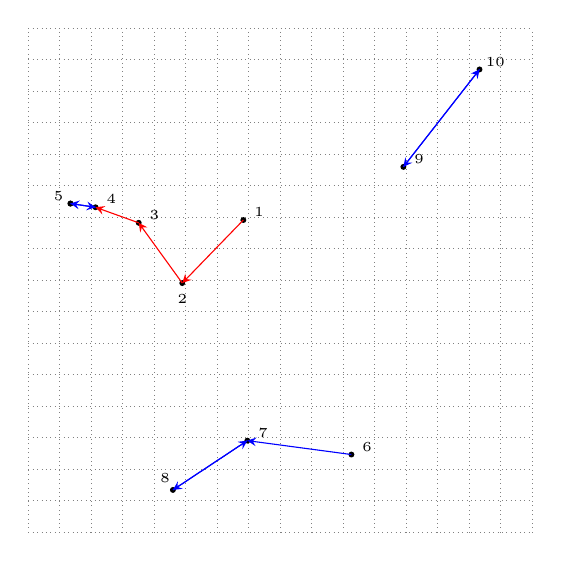
\begin{tikzpicture}[scale=1]
%		   \tkzInit[xmax=10,ymax=10,xmin=-6,ymin=-6]
%			\begin{scope}[scale=0.2,dash pattern=on 0.1pt off 0.5pt]
%			\tkzGrid
%			\end{scope}
%		   \tkzLabelX[orig=true,label options={font=\normalfont},step=1]
%		   \tkzLabelY[orig=false,label options={font=\normalfont}]
%		   \tkzDrawX[label={}] %right space=1.0,
%		   \tkzDrawY[label={}]
\begin{scope}[scale=2]

\tkzInit[xmax=10,ymax=10,xmin=-6,ymin=-6]
\begin{scope}[scale=0.2,dash pattern=on 0.1pt off 1.5pt]
\tkzGrid	
\end{scope}

\pointnnc[fill=black,draw] {0.16608544}{0.78196448}
\pointnnc[fill=black,draw] {-0.22178966}{0.38172358}
\pointnnc[fill=black,draw] {-0.49853725}{0.76432549}
\pointnnc[fill=black,draw] {-0.77257544}{0.86298719}
\pointnnc[fill=black,draw] {-0.93165719}{0.88666088}


%\Center[fill=black,draw] {1.18222626}{1.11937572}
\pointnnc[fill=black,draw] {0.85228509}{-0.70707096}
\pointnnc[fill=black,draw] {-0.93165719}{0.88666088}
\pointnnc[fill=black,draw] {-0.28126003}{-0.93192543}
\pointnnc[fill=black,draw] {0.19150443}{-0.61876383}
\pointnnc[fill=black,draw] {1.66571909}{1.7381882}
\pointnnc[fill=black,draw] {1.18222626}{1.11937572}

\node [xshift=0.2cm, yshift=0.1cm, font=\tiny] at (0.16608544,0.78196448) {1};
\node [xshift=0.0cm, yshift=-0.2cm, font=\tiny] at (-0.22178966,0.38172358) {2};
\node [xshift=0.2cm, yshift=0.1cm, font=\tiny] at (-0.49853725,0.76432549) {3};
\node [xshift=0.2cm, yshift=0.1cm, font=\tiny] at (-0.77257544,0.86298719) {4};
\node [xshift=-0.15cm, yshift=0.1cm, font=\tiny] at (-0.93165719,0.88666088) {5};

\node [xshift=0.2cm, yshift=0.1cm, font=\tiny] at (0.85228509,-0.70707096) {6};
\node [xshift=0.2cm, yshift=0.1cm, font=\tiny] at (0.19150443,-0.61876383) {7};
\node [xshift=-0.1cm, yshift=0.15cm, font=\tiny] at (-0.28126003,-0.93192543) {8};
\node [xshift=0.2cm, yshift=0.1cm, font=\tiny] at (1.18222626,1.11937572) {9};
\node [xshift=0.2cm, yshift=0.1cm, font=\tiny] at (1.66571909,1.7381882) {10};


\draw [arrow,draw=red] (0.16608544,0.78196448) -- (-0.22178966,0.38172358); %1-2
\draw [arrow,draw=red] (-0.22178966,0.38172358) --(-0.49853725,0.76432549); % 2-3
\draw [arrow,draw=red] (-0.49853725,0.76432549) -- (-0.77257544,0.86298719); % 3-4
\draw [arrow,draw=blue] (-0.77257544,0.86298719) -- (-0.93165719,0.88666088); % 4-5
\draw [arrow,draw=blue] (-0.93165719,0.88666088) --(-0.77257544,0.86298719); % 5-4

\draw [arrow,draw=blue] (0.85228509,-0.70707096) --(0.19150443,-0.61876383); % 6-7
\draw [arrow,draw=blue] (0.19150443,-0.61876383) --(-0.28126003,-0.93192543); % 7-8
\draw [arrow,draw=blue] (-0.28126003,-0.93192543) --(0.19150443,-0.61876383); % 8-7

\draw [arrow,draw=blue] (1.18222626,1.11937572) --(1.66571909,1.7381882); % 9-10
\draw [arrow,draw=blue] (1.66571909,1.7381882) --(1.18222626,1.11937572); % 10-9



%\draw (0,0) circle (0.03cm);

\end{scope}

		\end{tikzpicture}
\end{document}